%%%% Paramétrage du TD %%%%
\def\xxactivite{ \ifprof \normalsize{Application 1 -- Corrigé } \else  Application 1 \fi} % \normalsize \vspace{-.4cm}
\def\xxauteur{\textsl{Xavier Pessoles}}


\def\xxnumchapitre{Chapitre 1 \vspace{.2cm}}
\def\xxchapitre{\hspace{.12cm} Introduction à la dynamique du solide indéformable}

\def\xxcompetences{%
\textsl{%
\textbf{Savoirs et compétences :}\\
\begin{itemize}[label=\ding{112},font=\color{ocre}] 
\item \textit{Res1.C2} : principe fondamental de la dynamique;
\item \textit{Res1.C1.SF1} : proposer une démarche permettant la détermination de la loi de mouvement.
\end{itemize}
}}

\def\xxtitreexo{Application -- Pompe à plateau}%Motorisation du moteur Haibike}
\def\xxsourceexo{\hspace{.2cm} \footnotesize{C. Gamelon \& P. Dubois}}
%\def\xxauteur{\textsl{Xavier Pessoles}}

\def\xxfigures{
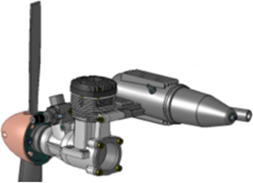
\includegraphics[width=.4\linewidth]{fig_00}
}%figues de la page de garde


\iflivret
\pagestyle{empty}


%%%%%%%% PAGE DE GARDE COURS
\ifcours
% ==== BANDEAU DES TITRES ==== 
\begin{tikzpicture}[remember picture,overlay]
\node at (current page.north west)
{\begin{tikzpicture}[remember picture,overlay]
\node[anchor=north west,inner sep=0pt] at (0,0) {\includegraphics[width=\paperwidth]{\thechapterimage}};
\draw[anchor=west] (-2cm,-8cm) node [line width=2pt,rounded corners=15pt,draw=ocre,fill=white,fill opacity=0.6,inner sep=40pt]{\strut\makebox[22cm]{}};
\draw[anchor=west] (1cm,-8cm) node {\huge\sffamily\bfseries\color{black} %
\begin{minipage}{1cm}
\rotatebox{90}{\LARGE\sffamily\textsc{\color{ocre}\textbf{\xxnumpartie}}}
\end{minipage} \hfill
\begin{minipage}[c]{14cm}
\begin{titrepartie}
\begin{flushright}
\renewcommand{\baselinestretch}{1.1} 
\Large\sffamily\textsc{\textbf{\xxpartie}}
\renewcommand{\baselinestretch}{1} 
\end{flushright}
\end{titrepartie}
\end{minipage} \hfill
\begin{minipage}[c]{3.5cm}
{\large\sffamily\textsc{\textbf{\color{ocre} \discipline}}}
\end{minipage} 
 };
\end{tikzpicture}};
\end{tikzpicture}
% ==== FIN BANDEAU DES TITRES ==== 


% ==== ONGLET 
\begin{tikzpicture}[overlay]
\node[shape=rectangle, 
      rounded corners = .25 cm,
	  draw= ocre,
	  line width=2pt, 
	  fill = ocre!10,
	  minimum width  = 2.5cm,
	  minimum height = 3cm,] at (18.3cm,0) {};
\node at (17.7cm,0) {\rotatebox{90}{\textbf{\Large\color{ocre}{\classe}}}};
%{};
\end{tikzpicture}
% ==== FIN ONGLET 


\vspace{3.5cm}

\begin{tikzpicture}[remember picture,overlay]
\draw[anchor=west] (-2cm,-6cm) node {\huge\sffamily\bfseries\color{black} %
\begin{minipage}{2cm}
\begin{center}
\LARGE\sffamily\textsc{\color{ocre}\textbf{\xxactivite}}
\end{center}
\end{minipage} \hfill
\begin{minipage}[c]{15cm}
\begin{titrechapitre}
\renewcommand{\baselinestretch}{1.1} 
\Large\sffamily\textsc{\textbf{\xxnumchapitre}}

\Large\sffamily\textsc{\textbf{\xxchapitre}}
\vspace{.5cm}

\renewcommand{\baselinestretch}{1} 
\normalsize\normalfont
\xxcompetences
\end{titrechapitre}
\end{minipage}  };
\end{tikzpicture}
\vfill

\begin{flushright}
\begin{minipage}[c]{.3\linewidth}
\begin{center}
\xxfigures
\end{center}
\end{minipage}\hfill
\begin{minipage}[c]{.6\linewidth}
\startcontents
%\printcontents{}{1}{}
\printcontents{}{1}{}
\end{minipage}
\end{flushright}

\begin{tikzpicture}[remember picture,overlay]
\draw[anchor=west] (4.5cm,-.7cm) node {
\begin{minipage}[c]{.2\linewidth}
\begin{flushright}

\includegraphics[width=2cm]{logoCC}
\end{flushright}
\end{minipage}
\begin{minipage}[c]{.2\linewidth}
\textsl{\xxauteur} \\
\textsl{\classe}
\end{minipage}
 };
\end{tikzpicture}

\newpage
\pagestyle{fancy}

%\newpage
%\pagestyle{fancy}

\else
\fi
%% FIN PAGE DE GARDE DES COURS

%%%%%%%% PAGE DE GARDE TD
\iftd
%\begin{tikzpicture}[remember picture,overlay]
%\node at (current page.north west)
%{\begin{tikzpicture}[remember picture,overlay]
%\draw[anchor=west] (-2cm,-3.25cm) node [line width=2pt,rounded corners=15pt,draw=ocre,fill=white,fill opacity=0.6,inner sep=40pt]{\strut\makebox[22cm]{}};
%\draw[anchor=west] (1cm,-3.25cm) node {\huge\sffamily\bfseries\color{black} %
%\begin{minipage}{1cm}
%\rotatebox{90}{\LARGE\sffamily\textsc{\color{ocre}\textbf{\xxnumpartie}}}
%\end{minipage} \hfill
%\begin{minipage}[c]{13.5cm}
%\begin{titrepartie}
%\begin{flushright}
%\renewcommand{\baselinestretch}{1.1} 
%\Large\sffamily\textsc{\textbf{\xxpartie}}
%\renewcommand{\baselinestretch}{1} 
%\end{flushright}
%\end{titrepartie}
%\end{minipage} \hfill
%\begin{minipage}[c]{3.5cm}
%{\large\sffamily\textsc{\textbf{\color{ocre} \discipline}}}
%\end{minipage} 
% };
%\end{tikzpicture}};
%\end{tikzpicture}

%%%%%%%%%% PAGE DE GARDE TD %%%%%%%%%%%%%%%
%\begin{tikzpicture}[overlay]
%\node[shape=rectangle, 
%      rounded corners = .25 cm,
%	  draw= ocre,
%	  line width=2pt, 
%	  fill = ocre!10,
%	  minimum width  = 2.5cm,
%	  minimum height = 2.5cm,] at (18.5cm,0) {};
%\node at (17.7cm,0) {\rotatebox{90}{\textbf{\Large\color{ocre}{\classe}}}};
%%{};
%\end{tikzpicture}

% PARTIE ET CHAPITRE
%\begin{tikzpicture}[remember picture,overlay]
%\draw[anchor=west] (-1cm,-2.1cm) node {\large\sffamily\bfseries\color{black} %
%\begin{minipage}[c]{15cm}
%\begin{flushleft}
%\xxnumchapitre \\
%\xxchapitre
%\end{flushleft}
%\end{minipage}  };
%\end{tikzpicture}

% BANDEAU EXO
\iflivret % SI LIVRET
\begin{tikzpicture}[remember picture,overlay]
\draw[anchor=west] (-2cm,-3.3cm) node {\huge\sffamily\bfseries\color{black} %
\begin{minipage}{5cm}
\begin{center}
\LARGE\sffamily\color{ocre}\textbf{\textsc{\xxactivite}}

\begin{center}
\xxfigures
\end{center}

\end{center}
\end{minipage} \hfill
\begin{minipage}[c]{12cm}
\begin{titrechapitre}
\renewcommand{\baselinestretch}{1.1} 
\large\sffamily\textbf{\textsc{\xxtitreexo}}

\small\sffamily{\textbf{\textit{\color{black!70}\xxsourceexo}}}
\vspace{.5cm}

\renewcommand{\baselinestretch}{1} 
\normalsize\normalfont
\xxcompetences
\end{titrechapitre}
\end{minipage}};
\end{tikzpicture}
\else % ELSE NOT LIVRET
\begin{tikzpicture}[remember picture,overlay]
\draw[anchor=west] (-2cm,-4.5cm) node {\huge\sffamily\bfseries\color{black} %
\begin{minipage}{5cm}
\begin{center}
\LARGE\sffamily\color{ocre}\textbf{\textsc{\xxactivite}}

\begin{center}
\xxfigures
\end{center}

\end{center}
\end{minipage} \hfill
\begin{minipage}[c]{12cm}
\begin{titrechapitre}
\renewcommand{\baselinestretch}{1.1} 
\large\sffamily\textbf{\textsc{\xxtitreexo}}

\small\sffamily{\textbf{\textit{\color{black!70}\xxsourceexo}}}
\vspace{.5cm}

\renewcommand{\baselinestretch}{1} 
\normalsize\normalfont
\xxcompetences
\end{titrechapitre}
\end{minipage}};
\end{tikzpicture}

\fi

\else   % FIN IF TD
\fi


%%%%%%%% PAGE DE GARDE FICHE
\iffiche
\begin{tikzpicture}[remember picture,overlay]
\node at (current page.north west)
{\begin{tikzpicture}[remember picture,overlay]
\draw[anchor=west] (-2cm,-2.25cm) node [line width=2pt,rounded corners=15pt,draw=ocre,fill=white,fill opacity=0.6,inner sep=40pt]{\strut\makebox[22cm]{}};
\draw[anchor=west] (1cm,-2.25cm) node {\huge\sffamily\bfseries\color{black} %
\begin{minipage}{1cm}
\rotatebox{90}{\LARGE\sffamily\textsc{\color{ocre}\textbf{\xxnumpartie}}}
\end{minipage} \hfill
\begin{minipage}[c]{14cm}
\begin{titrepartie}
\begin{flushright}
\renewcommand{\baselinestretch}{1.1} 
\large\sffamily\textsc{\textbf{\xxpartie} \\} 

\vspace{.2cm}

\normalsize\sffamily\textsc{\textbf{\xxnumchapitre -- \xxchapitre}}
\renewcommand{\baselinestretch}{1} 
\end{flushright}
\end{titrepartie}
\end{minipage} \hfill
\begin{minipage}[c]{3.5cm}
{\large\sffamily\textsc{\textbf{\color{ocre} \discipline}}}
\end{minipage} 
 };
\end{tikzpicture}};
\end{tikzpicture}

\iflivret
\begin{tikzpicture}[overlay]
\node[shape=rectangle, 
      rounded corners = .25 cm,
	  draw= ocre,
	  line width=2pt, 
	  fill = ocre!10,
	  minimum width  = 2.5cm,
	  minimum height = 2.5cm,] at (18.5cm,.5cm) {};
\node at (17.9cm,.5cm) {\rotatebox{90}{\textsf{\textbf{\large\color{ocre}{\classe}}}}};
%{};
\end{tikzpicture}
\else
\begin{tikzpicture}[overlay]
\node[shape=rectangle, 
      rounded corners = .25 cm,
	  draw= ocre,
	  line width=2pt, 
	  fill = ocre!10,
	  minimum width  = 2.5cm,
%	  minimum height = 2.5cm,] at (18.5cm,1.1cm) {};
	  minimum height = 2.5cm,] at (18.6cm,0.5cm) {};
\node at (18cm,0.5cm) {\rotatebox{90}{\textsf{\textbf{\large\color{ocre}{\classe}}}}};
%{};
\end{tikzpicture}

\fi

\else
\fi



\else
\pagestyle{empty}


%%%%%%%% PAGE DE GARDE COURS
\ifcours
% ==== BANDEAU DES TITRES ==== 
\begin{tikzpicture}[remember picture,overlay]
\node at (current page.north west)
{\begin{tikzpicture}[remember picture,overlay]
\node[anchor=north west,inner sep=0pt] at (0,0) {\includegraphics[width=\paperwidth]{\thechapterimage}};
\draw[anchor=west] (-2cm,-8cm) node [line width=2pt,rounded corners=15pt,draw=ocre,fill=white,fill opacity=0.6,inner sep=40pt]{\strut\makebox[22cm]{}};
\draw[anchor=west] (1cm,-8cm) node {\huge\sffamily\bfseries\color{black} %
\begin{minipage}{1cm}
\rotatebox{90}{\LARGE\sffamily\textsc{\color{ocre}\textbf{\xxnumpartie}}}
\end{minipage} \hfill
\begin{minipage}[c]{14cm}
\begin{titrepartie}
\begin{flushright}
\renewcommand{\baselinestretch}{1.1} 
\Large\sffamily\textsc{\textbf{\xxpartie}}
\renewcommand{\baselinestretch}{1} 
\end{flushright}
\end{titrepartie}
\end{minipage} \hfill
\begin{minipage}[c]{3.5cm}
{\large\sffamily\textsc{\textbf{\color{ocre} \discipline}}}
\end{minipage} 
 };
\end{tikzpicture}};
\end{tikzpicture}
% ==== FIN BANDEAU DES TITRES ==== 


% ==== ONGLET 
\begin{tikzpicture}[overlay]
\node[shape=rectangle, 
      rounded corners = .25 cm,
	  draw= ocre,
	  line width=2pt, 
	  fill = ocre!10,
	  minimum width  = 2.5cm,
	  minimum height = 3cm,] at (18.3cm,0) {};
\node at (17.7cm,0) {\rotatebox{90}{\textbf{\Large\color{ocre}{\classe}}}};
%{};
\end{tikzpicture}
% ==== FIN ONGLET 


\vspace{3.5cm}

\begin{tikzpicture}[remember picture,overlay]
\draw[anchor=west] (-2cm,-6cm) node {\huge\sffamily\bfseries\color{black} %
\begin{minipage}{2cm}
\begin{center}
\LARGE\sffamily\textsc{\color{ocre}\textbf{\xxactivite}}
\end{center}
\end{minipage} \hfill
\begin{minipage}[c]{15cm}
\begin{titrechapitre}
\renewcommand{\baselinestretch}{1.1} 
\Large\sffamily\textsc{\textbf{\xxnumchapitre}}

\Large\sffamily\textsc{\textbf{\xxchapitre}}
\vspace{.5cm}

\renewcommand{\baselinestretch}{1} 
\normalsize\normalfont
\xxcompetences
\end{titrechapitre}
\end{minipage}  };
\end{tikzpicture}
\vfill

\begin{flushright}
\begin{minipage}[c]{.3\linewidth}
\begin{center}
\xxfigures
\end{center}
\end{minipage}\hfill
\begin{minipage}[c]{.6\linewidth}
\startcontents
%\printcontents{}{1}{}
\printcontents{}{1}{}
\end{minipage}
\end{flushright}

\begin{tikzpicture}[remember picture,overlay]
\draw[anchor=west] (4.5cm,-.7cm) node {
\begin{minipage}[c]{.2\linewidth}
\begin{flushright}

\includegraphics[width=2cm]{logoCC}
\end{flushright}
\end{minipage}
\begin{minipage}[c]{.2\linewidth}
\textsl{\xxauteur} \\
\textsl{\classe}
\end{minipage}
 };
\end{tikzpicture}

\newpage
\pagestyle{fancy}

%\newpage
%\pagestyle{fancy}

\else
\fi
%% FIN PAGE DE GARDE DES COURS

%%%%%%%% PAGE DE GARDE TD
\iftd
%\begin{tikzpicture}[remember picture,overlay]
%\node at (current page.north west)
%{\begin{tikzpicture}[remember picture,overlay]
%\draw[anchor=west] (-2cm,-3.25cm) node [line width=2pt,rounded corners=15pt,draw=ocre,fill=white,fill opacity=0.6,inner sep=40pt]{\strut\makebox[22cm]{}};
%\draw[anchor=west] (1cm,-3.25cm) node {\huge\sffamily\bfseries\color{black} %
%\begin{minipage}{1cm}
%\rotatebox{90}{\LARGE\sffamily\textsc{\color{ocre}\textbf{\xxnumpartie}}}
%\end{minipage} \hfill
%\begin{minipage}[c]{13.5cm}
%\begin{titrepartie}
%\begin{flushright}
%\renewcommand{\baselinestretch}{1.1} 
%\Large\sffamily\textsc{\textbf{\xxpartie}}
%\renewcommand{\baselinestretch}{1} 
%\end{flushright}
%\end{titrepartie}
%\end{minipage} \hfill
%\begin{minipage}[c]{3.5cm}
%{\large\sffamily\textsc{\textbf{\color{ocre} \discipline}}}
%\end{minipage} 
% };
%\end{tikzpicture}};
%\end{tikzpicture}

%%%%%%%%%% PAGE DE GARDE TD %%%%%%%%%%%%%%%
%\begin{tikzpicture}[overlay]
%\node[shape=rectangle, 
%      rounded corners = .25 cm,
%	  draw= ocre,
%	  line width=2pt, 
%	  fill = ocre!10,
%	  minimum width  = 2.5cm,
%	  minimum height = 2.5cm,] at (18.5cm,0) {};
%\node at (17.7cm,0) {\rotatebox{90}{\textbf{\Large\color{ocre}{\classe}}}};
%%{};
%\end{tikzpicture}

% PARTIE ET CHAPITRE
%\begin{tikzpicture}[remember picture,overlay]
%\draw[anchor=west] (-1cm,-2.1cm) node {\large\sffamily\bfseries\color{black} %
%\begin{minipage}[c]{15cm}
%\begin{flushleft}
%\xxnumchapitre \\
%\xxchapitre
%\end{flushleft}
%\end{minipage}  };
%\end{tikzpicture}

% BANDEAU EXO
\iflivret % SI LIVRET
\begin{tikzpicture}[remember picture,overlay]
\draw[anchor=west] (-2cm,-3.3cm) node {\huge\sffamily\bfseries\color{black} %
\begin{minipage}{5cm}
\begin{center}
\LARGE\sffamily\color{ocre}\textbf{\textsc{\xxactivite}}

\begin{center}
\xxfigures
\end{center}

\end{center}
\end{minipage} \hfill
\begin{minipage}[c]{12cm}
\begin{titrechapitre}
\renewcommand{\baselinestretch}{1.1} 
\large\sffamily\textbf{\textsc{\xxtitreexo}}

\small\sffamily{\textbf{\textit{\color{black!70}\xxsourceexo}}}
\vspace{.5cm}

\renewcommand{\baselinestretch}{1} 
\normalsize\normalfont
\xxcompetences
\end{titrechapitre}
\end{minipage}};
\end{tikzpicture}
\else % ELSE NOT LIVRET
\begin{tikzpicture}[remember picture,overlay]
\draw[anchor=west] (-2cm,-4.5cm) node {\huge\sffamily\bfseries\color{black} %
\begin{minipage}{5cm}
\begin{center}
\LARGE\sffamily\color{ocre}\textbf{\textsc{\xxactivite}}

\begin{center}
\xxfigures
\end{center}

\end{center}
\end{minipage} \hfill
\begin{minipage}[c]{12cm}
\begin{titrechapitre}
\renewcommand{\baselinestretch}{1.1} 
\large\sffamily\textbf{\textsc{\xxtitreexo}}

\small\sffamily{\textbf{\textit{\color{black!70}\xxsourceexo}}}
\vspace{.5cm}

\renewcommand{\baselinestretch}{1} 
\normalsize\normalfont
\xxcompetences
\end{titrechapitre}
\end{minipage}};
\end{tikzpicture}

\fi

\else   % FIN IF TD
\fi


%%%%%%%% PAGE DE GARDE FICHE
\iffiche
\begin{tikzpicture}[remember picture,overlay]
\node at (current page.north west)
{\begin{tikzpicture}[remember picture,overlay]
\draw[anchor=west] (-2cm,-2.25cm) node [line width=2pt,rounded corners=15pt,draw=ocre,fill=white,fill opacity=0.6,inner sep=40pt]{\strut\makebox[22cm]{}};
\draw[anchor=west] (1cm,-2.25cm) node {\huge\sffamily\bfseries\color{black} %
\begin{minipage}{1cm}
\rotatebox{90}{\LARGE\sffamily\textsc{\color{ocre}\textbf{\xxnumpartie}}}
\end{minipage} \hfill
\begin{minipage}[c]{14cm}
\begin{titrepartie}
\begin{flushright}
\renewcommand{\baselinestretch}{1.1} 
\large\sffamily\textsc{\textbf{\xxpartie} \\} 

\vspace{.2cm}

\normalsize\sffamily\textsc{\textbf{\xxnumchapitre -- \xxchapitre}}
\renewcommand{\baselinestretch}{1} 
\end{flushright}
\end{titrepartie}
\end{minipage} \hfill
\begin{minipage}[c]{3.5cm}
{\large\sffamily\textsc{\textbf{\color{ocre} \discipline}}}
\end{minipage} 
 };
\end{tikzpicture}};
\end{tikzpicture}

\iflivret
\begin{tikzpicture}[overlay]
\node[shape=rectangle, 
      rounded corners = .25 cm,
	  draw= ocre,
	  line width=2pt, 
	  fill = ocre!10,
	  minimum width  = 2.5cm,
	  minimum height = 2.5cm,] at (18.5cm,.5cm) {};
\node at (17.9cm,.5cm) {\rotatebox{90}{\textsf{\textbf{\large\color{ocre}{\classe}}}}};
%{};
\end{tikzpicture}
\else
\begin{tikzpicture}[overlay]
\node[shape=rectangle, 
      rounded corners = .25 cm,
	  draw= ocre,
	  line width=2pt, 
	  fill = ocre!10,
	  minimum width  = 2.5cm,
%	  minimum height = 2.5cm,] at (18.5cm,1.1cm) {};
	  minimum height = 2.5cm,] at (18.6cm,0.5cm) {};
\node at (18cm,0.5cm) {\rotatebox{90}{\textsf{\textbf{\large\color{ocre}{\classe}}}}};
%{};
\end{tikzpicture}

\fi

\else
\fi



\fi
\setlength{\columnseprule}{.1pt}

\pagestyle{fancy}
\thispagestyle{plain}

\ifprof
\vspace{5.5cm}
\else
\vspace{4.9cm}
\fi

\def\columnseprulecolor{\color{ocre}}
\setlength{\columnseprule}{0.4pt} 

%%%%%%%%%%%%%%%%%%%%%%%

\setcounter{exo}{0}



\ifprof
%\begin{multicols}{2}
\else
\begin{multicols}{2}
\fi


\ifprof
\else

Considérons le mécanisme de pompe représenté sur la figure ci-dessous.

\begin{center}
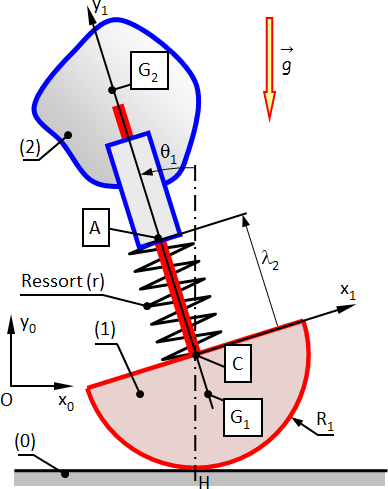
\includegraphics[width=\linewidth]{fig_01}
\end{center}


\begin{center}
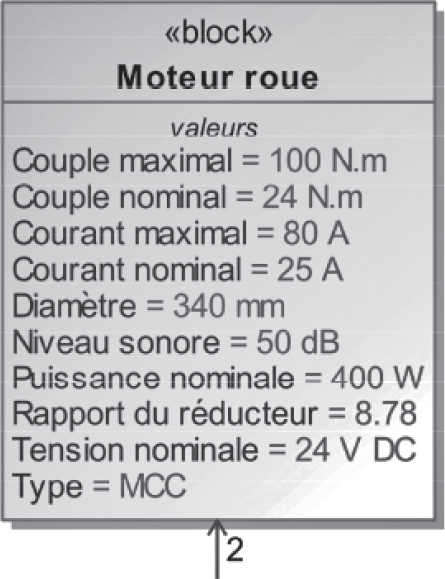
\includegraphics[width=\linewidth]{fig_02}
\end{center}

L'arbre excentrique \textbf{(1)}, animé d'un mouvement de rotation autour de l'axe $\axe{O}{x_0}$  horizontal, agit sur le piston \textbf{(2)} en liaison pivot glissant d'axe $\axe{O}{z_0}$ avec le bâti \textbf{(0)}. Pendant la phase de descente du piston \textbf{(2)}, le contact ponctuel en $I$ avec l’excentrique est maintenu par un ressort \textbf{(r)}.

\subsection*{Paramétrage}
Le repère $\repere{O}{x_0}{y_0}{z_0}$ lié au bâti \textbf{(0)} est supposé galiléen.
Le repère $\repere{O}{x_1}{y_1}{z_1}$ est lié à l'arbre excentrique \textbf{(1)}.
On a de plus :
\begin{itemize}
\item $\angl{y_0}{y_1}=\angl{z_0}{z_1}=\theta$;
\item $\vect{OB}=e\vect{z_1}$;
\item $\vect{BI}=R\vect{z_0}$;
\item $\vect{OA}=z\vect{z_0}$. 
\end{itemize} 	 	 		 
Les liaisons pivot entre \textbf{(0)} et \textbf{(1)}, ponctuelle entre \textbf{(1)} et \textbf{(2)}, et pivot glissant entre \textbf{(0)} et \textbf{(2)} sont supposées sans frottement.
Le solide \textbf{(1)} possède un moment d’inertie $I_1$ par rapport à l'axe $\axe{O}{x_0}$. Le piston \textbf{(2)} possède une masse $m_2$.
Le ressort \textbf{(r)}, de raideur $k$, est toujours comprimé. Pour $\theta = \pm \dfrac{\pi}{2}$, l'effort de compression est égal à $\vect{F_0}=-F_0\vect{z_0}$.
Un moteur exerce un couple connu de moment $\vect{C_m}=C_m\vect{x_0}$ sur l'arbre \textbf{(1)}. Le fluide exerce sur le piston une action connue, représentée par un glisseur d'axe $\axe{O}{z_0}$ et de résultante $\vect{F_h}=-F_h{\vect{z_0}}$.

\subparagraph{}\textit{En utilisant une fermeture géométrique ou la méthode de votre choix, déterminer la exprimer $z$ en fonction de $\theta$ et de constantes du problème. Déterminer alors $\vectv{A}{2}{0}$ et $\vectg{A}{2}{0}$.}

\subparagraph{}\textit{Proposer une méthode permettant de déterminer l'équation différentielle du mouvement relative au paramètre $\theta$ en utilisant le PFD.}


\subparagraph{}\textit{Mettre en  \oe{}uvre la méthode proposée précédemment.}

%\subparagraph{}\textit{Avec le théorème de l'énergie cinétique, déterminer l'équation différentielle du mouvement.}

\subparagraph{}\textit{En considérant un frottement sec au niveau de la liaison ponctuelle entre \textbf{(1)} et \textbf{(2)}, déterminer l'équation différentielle du mouvement.}


\ifprof
\else
\end{multicols}
\fi

\fi 
\ifprof
%\newpage

%TO DO : graphe de liaisons.
\textbf{Fermeture géométrique.}

On a : $\vect{OB}+\vect{BI}+\vect{IA}+\vect{AO}=\vect{0}$.

En projection sur $\vect{z_0}$ : $e\cos\theta+R=z$. Par dérivation successive, on a :
$-e\dot{\theta}\sin\theta=\dot{z}$ et $-e\ddot{\theta}\sin\theta-e\dot{\theta}^2\cos\theta=\ddot{z}$.


\textbf{On isole le solide \textbf{(1)}.}

\textbf{On réalise le bilan des actions mécaniques.}
\begin{itemize}
\item Liaison pivot : $\torseurstat{T}{0}{1}
=\torseurl{X_{01}\vect{x_0}+Y_{01}\vect{y_0}+Z_{01}\vect{z_0}}{M_{01}\vect{y_0}+N_{01}\vect{z_0}}{O}
=\torseurl{Y_{01}\vect{y_0}+Z_{01}\vect{z_0}}{\vect{0}}{O}$.
\item Liaison ponctuelle : $\torseurstat{T}{2}{1}
=\torseurl{Y_{21}\vect{y_0}+Z_{21}\vect{z_0}}{\vect{0}}{I}$. On a $Z_{21}<0$, $Y_{21}>0$ et à la limite du glissement, $Y_{21}=-fZ_{21}$. 

$\vectm{O}{2}{1}=\vectm{I}{2}{1}+\vect{OI}\wedge \vectf{2}{1}=\left( e\vect{z_1}+R\vect{z_0}\right)\wedge \left(Y_{21}\vect{y_0}+Z_{21}\vect{z_0} \right)$ 
$= -eY_{21}\cos\theta \vect{x_0}-e Z_{21}\sin\theta\vect{x_0}-RY_{21}\vect{x_0}$
$= -\left(\left(e\cos\theta+R\right)Y_{21} +e Z_{21}\sin\theta\right)\vect{x_0}$.

\item Couple moteur : $\torseurstat{T}{\text{Moteur}}{1}
=\torseurl{\vect{0}}{C_m\vect{x_0}}{O}$.
\end{itemize}

\textbf{Calcul de $\vectmd{O}{1}{0}\cdot \vect{x_0}$.}
 
$O$ est un point fixe et $I_1$ moment d'inertie par rapport à $\axe{O}{x_0}$ on a donc : 
$\vectmd{O}{1}{0}\cdot \vect{x_0}
=\left[\dfrac{\dd \vectmc{O}{1}{0}}{\dd t}\right]_{\mathcal{R}_0}\vect{x_0}
=\left[\dfrac{\dd \vectmc{O}{1}{0}\cdot \vect{x_0}}{\dd t}  \right]_{\mathcal{R}_0}$
$=\left[\dfrac{\dd \inertie{O}{1}\vecto{1}{0}\cdot \vect{x_0}}{\dd t}  \right]_{\mathcal{R}_0}$
$=\left[\dfrac{\dd I_1\dot{\theta}\vect{x_0}\cdot \vect{x_0}}{\dd t}  \right]_{\mathcal{R}_0}$
$=I_1\ddot{\theta}$.

\textbf{Application du théorème du moment dynamique en projection sur $\vect{x_0}$.}
$$
C_m-\left(\left(e\cos\theta+R\right)Y_{21} +e Z_{21}\sin\theta\right) =I_1\ddot{\theta}.
$$

\textbf{On isole le solide \textbf{(2)}.}

\textbf{On réalise le bilan des actions mécaniques.}
\begin{itemize}
\item Liaison pivot glissant: $\torseurstat{T}{0}{2}
=\torseurl{Y_{02}\vect{y_0}}{L_{02}\vect{x_0}}{O}$.
\item Liaison ponctuelle : $\torseurstat{T}{1}{2}=-\torseurstat{T}{2}{1}
=\torseurl{-Y_{21}\vect{y_0}-Z_{21}\vect{z_0}}{\vect{0}}{I}$. 
\item Ressort: $\torseurstat{T}{\text{Ressort}}{2}
=\torseurl{-F_0-kz\vect{z_0}}{\vect{0}}{A}$.
\item Pesanteur: $\torseurstat{T}{\text{Pesanteur}}{2}
=\torseurl{-m_2g\vect{z_0}}{\vect{0}}{A}$.
\item Fluide: $\torseurstat{T}{\text{Fluide}}{2}
=\torseurl{-F_h\vect{z_0}}{\vect{0}}{A}$.

\end{itemize}

\textbf{Calcul de $\vectrd{2}{0}\cdot \vect{z_0}$.}
 
$\vectrd{2}{0}\cdot \vect{z_0}=m_2\ddot{z}$

\textbf{Application du théorème de la résultante dynamique en projection sur $\vect{z_0}$.}
$$
-F_h-Z_{21}-F_0-kz-m_2g=m_2\ddot{z}.
$$


\textbf{Bilan :}
$$C_m-\left(\left(e\cos\theta+R\right)Y_{21} +e \left( -F_h-F_0-kz-m_2g-m_2\ddot{z}\right)\sin\theta\right) =I_1\ddot{\theta}.$$

On a alors :
$$C_m-\left(\left(e\cos\theta+R\right)Y_{21} -e \left( F_h+F_0+k\left( e\cos\theta+R \right)+m_2g-em_2\left( \ddot{\theta}\sin\theta+\dot{\theta}^2\cos\theta\right)\right)\sin\theta\right) =I_1\ddot{\theta}.$$


\textbf{Bilan sans frottement :}
$$C_m+e\left(
F_h+F_0+k\left( e\cos\theta+R \right)+m_2g
-em_2\sin\theta\left( \ddot{\theta}\sin\theta+\dot{\theta}^2\cos\theta\right)
\right) =I_1\ddot{\theta}.$$
\else
\fi
